\documentclass[12pt]{article}

\usepackage{tikz}
\usepackage{geometry}

\usetikzlibrary{mindmap}

\pagestyle{empty}

\geometry{landscape, margin=1cm}


\begin{document}
\begin{center}
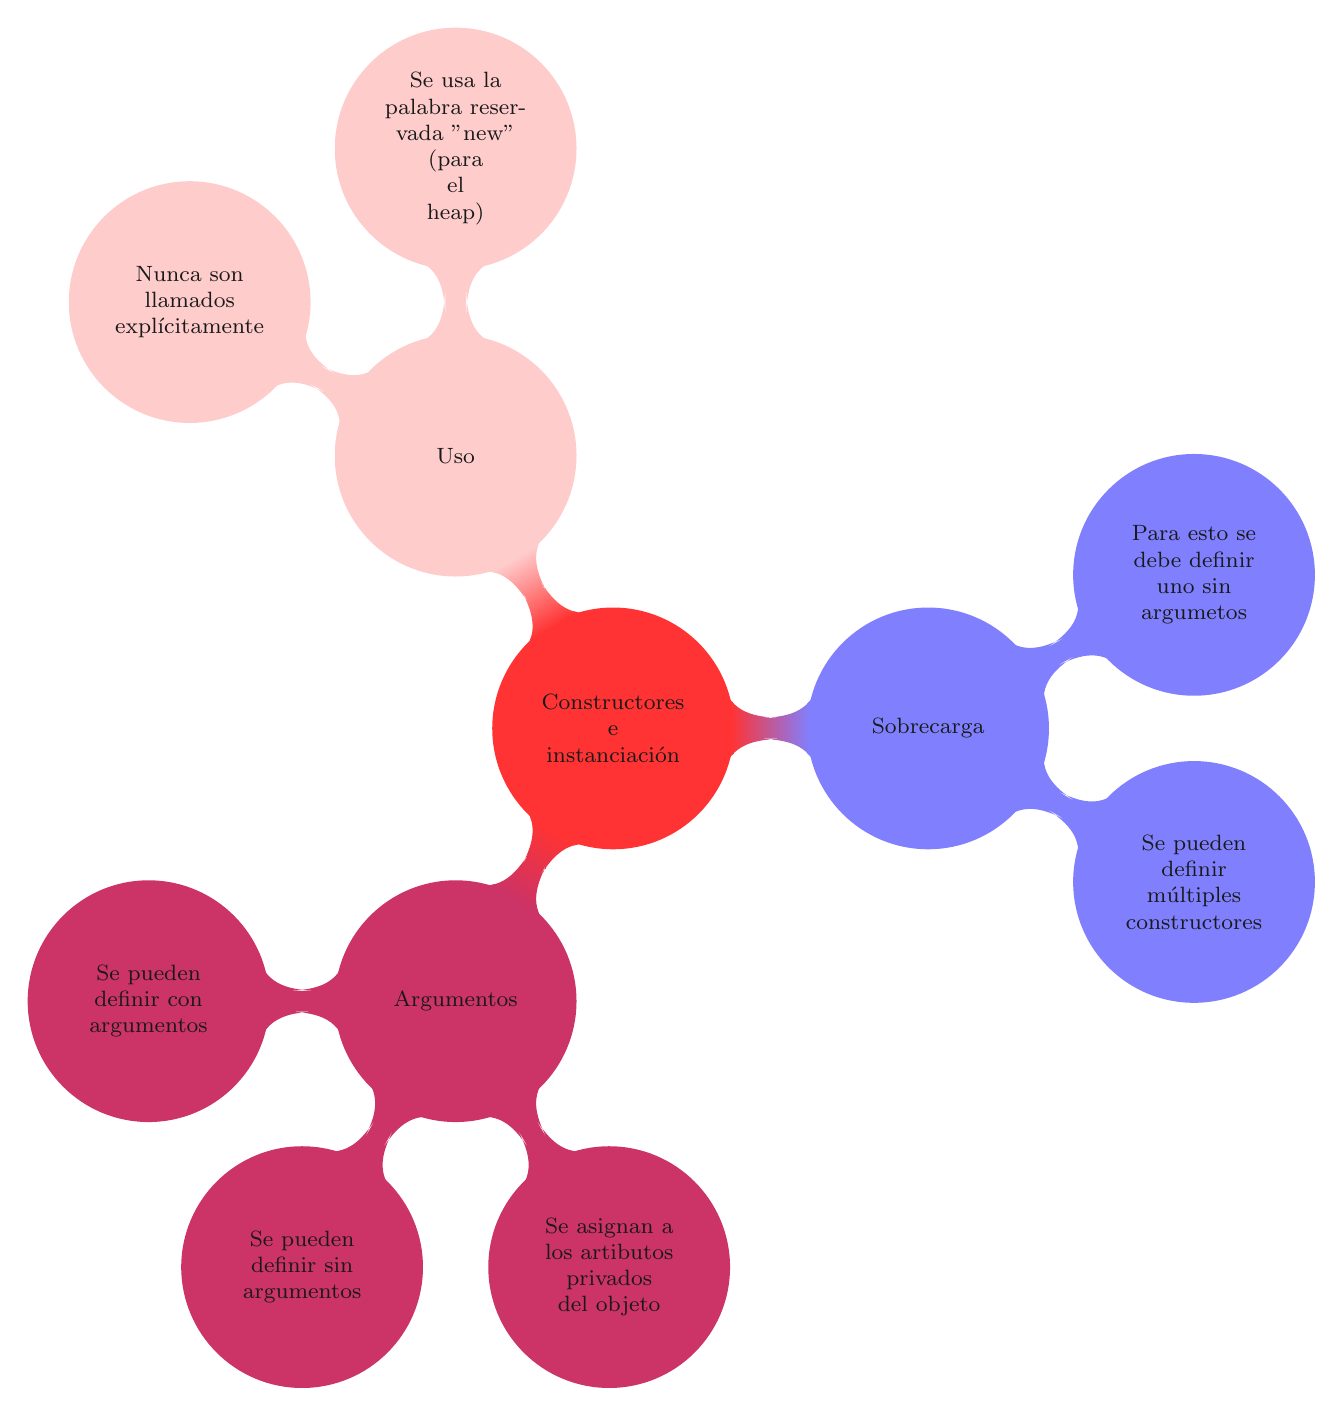
\begin{tikzpicture}[small mindmap, grow cyclic, every node/.style=concept, concept color=red!80, text=black!90, minimum size=3.0cm,
    level 1/.style={level distance=4.5cm,sibling angle=360/4},
    level 1/.style={level distance=4.0cm,sibling angle=360/3},
    level 2/.style={level distance=3.9cm,sibling angle=60},
    level 3/.style={level distance=3.5cm,sibling angle=60},
    ]

    \node{Constructores\\e\\instanciación}
    child[concept color=purple!80] { node {Argumentos}
        child { node {Se pueden definir con argumentos} }
        child { node {Se pueden definir sin argumentos} }
        child { node {Se asignan a los artibutos privados del objeto} }
    }
    child[concept color=blue!50] { node {Sobrecarga}
        child { node {Se pueden definir múltiples constructores} }
        child { node {Para esto se debe definir uno sin argumetos} }
    }
    child[concept color=pink!80] { node {Uso}
        child { node {Se usa la palabra reservada "new"\\(para\\el\\heap)} }
        child { node {Nunca son llamados explícitamente} }
    }

    ;
\end{tikzpicture}
\end{center}
\end{document}
